%!TEX root = ../../prace.tex

\section{Přepínač}

Přepínač slouží jako ovládání pro světla a~plničku

\begin{figure}[!ht]\centering
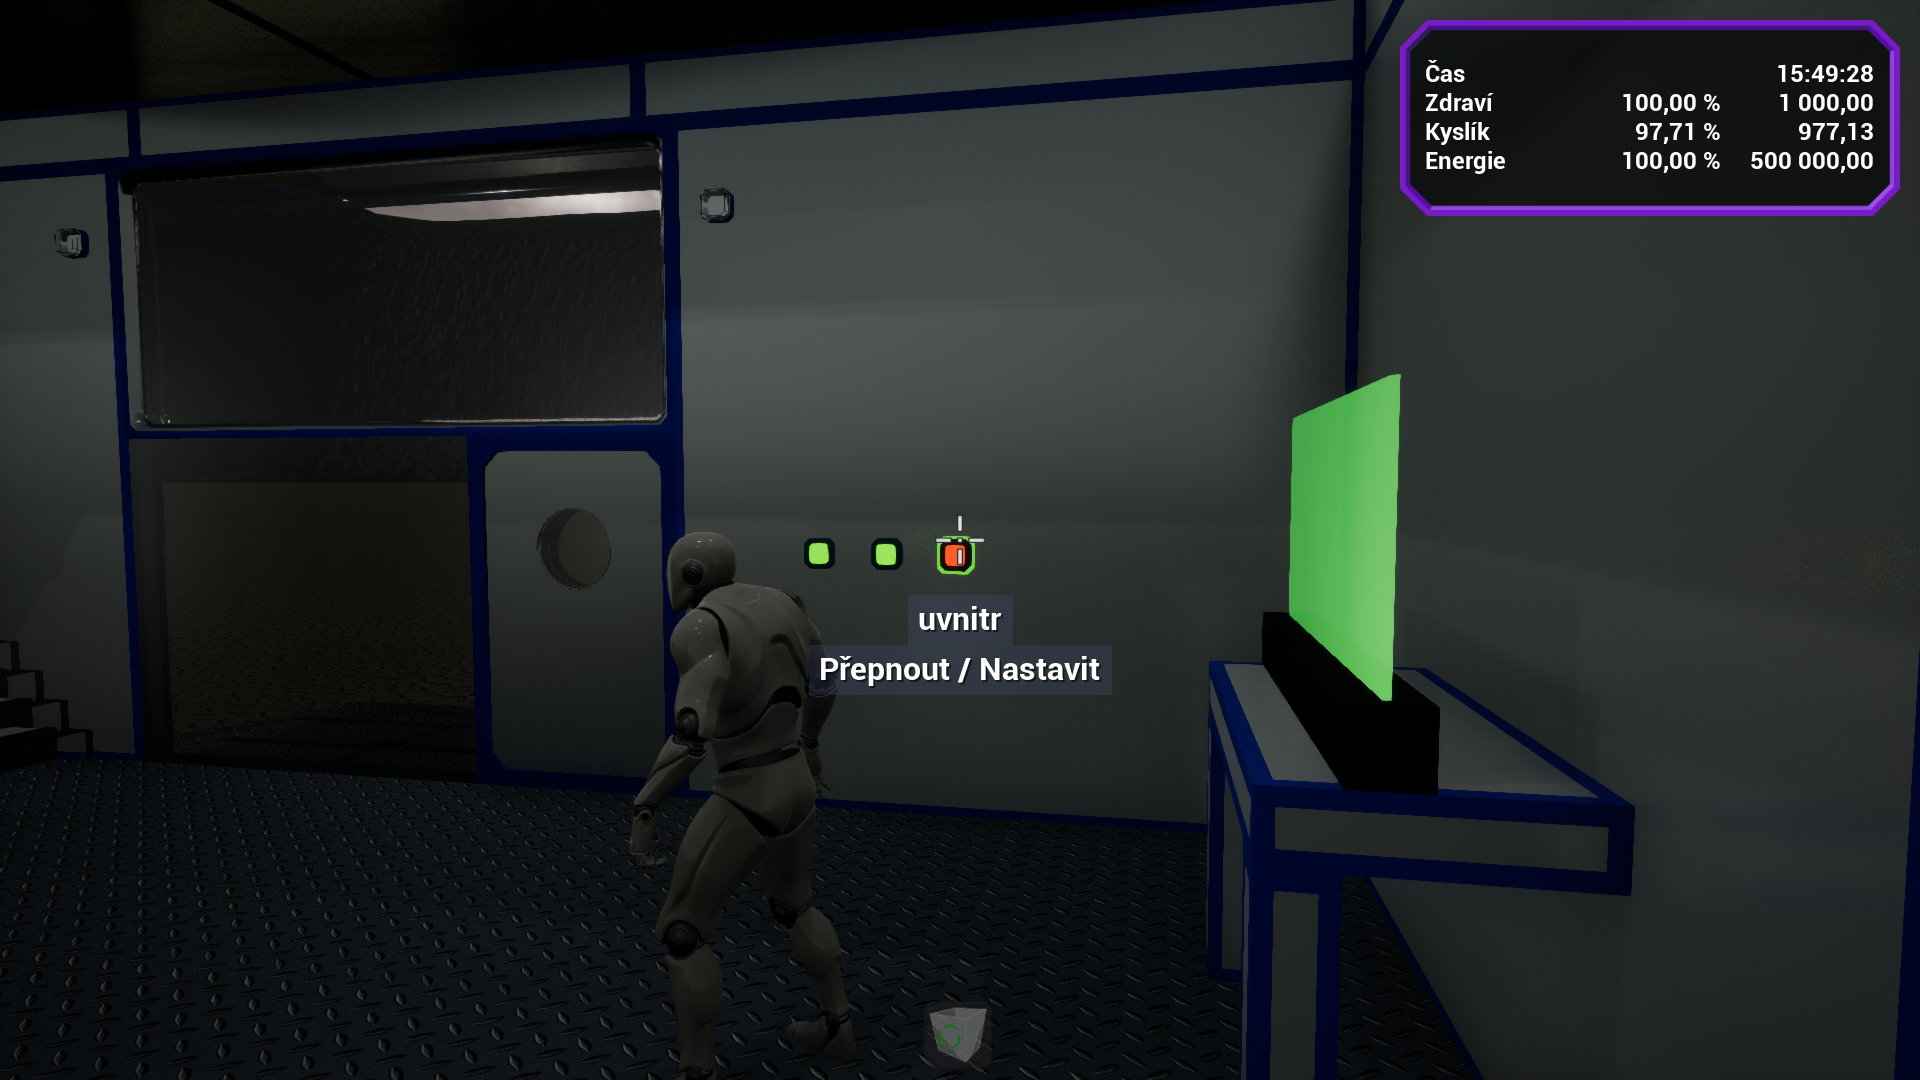
\includegraphics[ width=140mm]{../../img/user/switcher/0switcherGeneral}

\caption{Přepínač - den}
\label{fig:user_switcher_0switcherGeneral}

\end{figure}

\FloatBarrier

Blok umožňuje reagovat na denní dobu - automatické přepínání na definovaný stav, pokud začne den, nebo začne noc.

V levé části le možné přiřazovat ovládané bloky

\begin{figure}[!ht]\centering
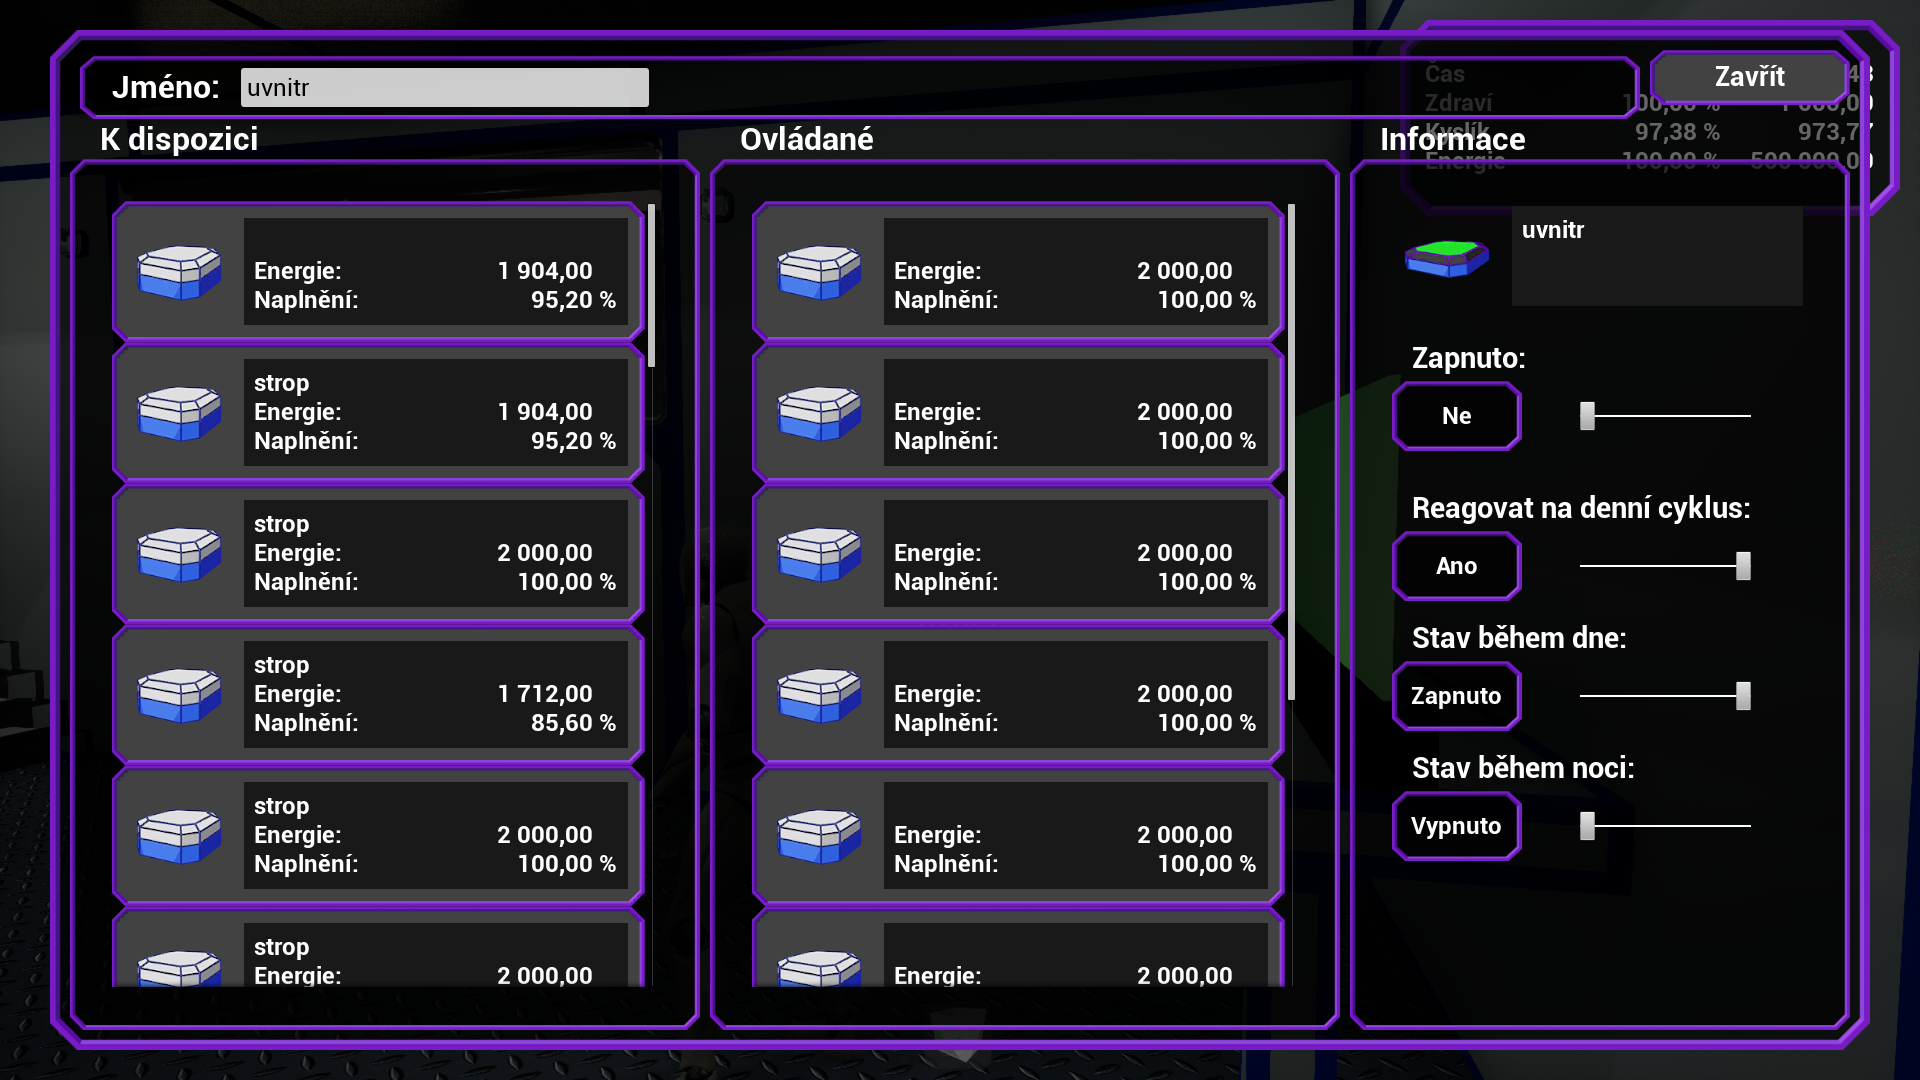
\includegraphics[ width=140mm]{../../img/user/switcher/switcherControls}

\caption{Přepínač - poledne, zataženo}
\label{fig:user_switcher_switcherControls}

\end{figure}


\FloatBarrier